% Created 2019-07-31 Wed 15:15
% Intended LaTeX compiler: pdflatex
\documentclass[presentation]{beamer}
\usepackage[utf8]{inputenc}
\usepackage[T1]{fontenc}
\usepackage{graphicx}
\usepackage{grffile}
\usepackage{longtable}
\usepackage{wrapfig}
\usepackage{rotating}
\usepackage[normalem]{ulem}
\usepackage{amsmath}
\usepackage{textcomp}
\usepackage{amssymb}
\usepackage{capt-of}
\usepackage{hyperref}
\usepackage[newfloat]{minted}
\usepackage{caption}
\usetheme{default}
\author{Yi Zhang, William R. Gillespie}
\date{\today}
\title{Population solvers in Torsten}
\hypersetup{
 pdfauthor={Yi Zhang, William R. Gillespie},
 pdftitle={Population solvers in Torsten},
 pdfkeywords={},
 pdfsubject={},
 pdfcreator={Emacs 25.3.1 (Org mode 9.1.3)}, 
 pdflang={English}}
\begin{document}

\maketitle

\begin{frame}[fragile,label={sec:org716192a}]{PMX population solvers}
 \begin{center}
\begin{tabular}{ll}
Single ODE system & ODE group\\
\hline
\texttt{pmx\_solve\_rk45} & \texttt{pmx\_solve\_group\_rk45}\\
\texttt{pmx\_solve\_bdf} & \texttt{pmx\_solve\_group\_bdf}\\
\texttt{pmx\_solve\_adams} & \texttt{pmx\_solve\_group\_adams}\\
\end{tabular}

\end{center}

\begin{columns}
\begin{column}{0.45\columnwidth}
\begin{block}{Individual solvers}
\begin{minted}[breaklines=true,fontsize=\footnotesize,breakanywhere=true]{stan}
matrix
pmx_solve_bdf(f, int nCmt,
  real[] time, real[] amt,
  real[] rate, real[] ii,
  int[] evid, int[] cmt,
  real[] addl, int[] ss,
  real[] theta, real[] biovar,
  real[] tlag, real rel_tol,
  real abs_tol, int max_step);
\end{minted}
\end{block}
\end{column}

\begin{column}{0.55\columnwidth}
\begin{block}{Population solvers}
\begin{minted}[breaklines=true,fontsize=\footnotesize,breakanywhere=true]{stan}
matrix
pmx_solve_group_bdf(f, int nCmt,
  int[] len, real[] time,
  real[] amt, real[] rate,
  real[] ii, int[] evid,
  int[] cmt, real[] addl,
  int[] ss, real[ , ] theta,
  real[ , ] biovar, real[ , ] tlag,
  real rel_tol, real abs_tol,
  int max_step);
\end{minted}
\end{block}
\end{column}
\end{columns}
\end{frame}


\begin{frame}[fragile,label={sec:org1590fdd}]{PMX population solvers}
 \begin{minted}[breaklines=true,fontsize=\footnotesize,breakanywhere=true]{stan}
matrix
pmx_solve_group_bdf(f, int nCmt, int[] len, real[] time, real[] amt, real[] rate, real[] ii, int[] evid, int[] cmt, real[] addl, int[] ss, real[,] theta, real[,] biovar, real[,] tlag, real rel_tol, real abs_tol, int max_step);
\end{minted}

\begin{block}{}
\begin{figure}[htbp]
\centering
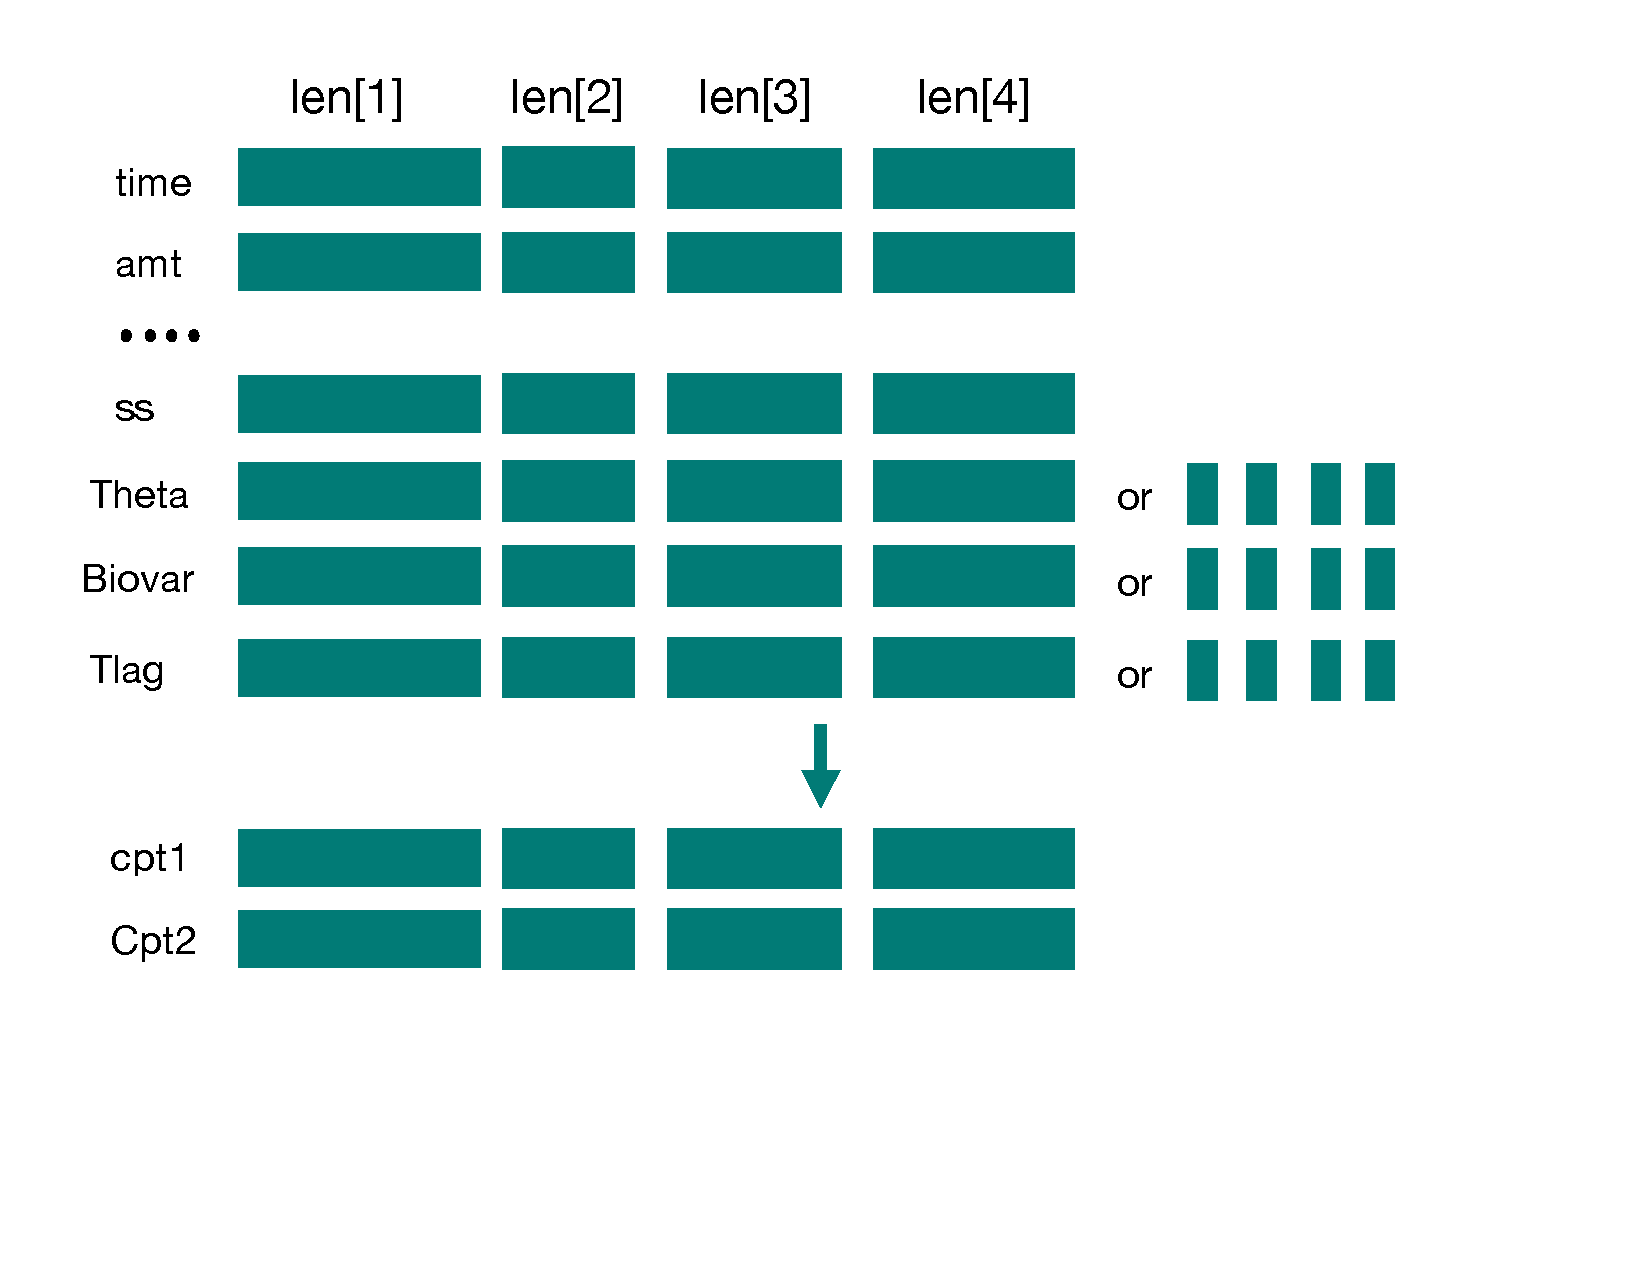
\includegraphics[width=0.6\textwidth]{./group_solver_args.pdf}
\caption{arguments and output of \texttt{pmx\_solve\_group\_xxx}}
\end{figure}
\end{block}
\end{frame}

\begin{frame}[label={sec:orga9077cb}]{Exercise}
We analyze the time to the first grade 2+ peripheral neuropathy
(PN) event in patients treated with an antibody-drug conjugate (ADC) delivering monomethyl auristatin E
(MMAE). We will simulate and analyze data using a simplified version of the
model reported in \cite{lu_time--event_2017}.
\begin{itemize}
\item Fauxlatuzumab vedotin 1.2 mg/kg IV boluses q3w \(\times\) 6 does.
\item 19 patients with 6 right-censored (simulated data).
\end{itemize}
\begin{columns}
\begin{column}{0.3\columnwidth}
\begin{block}{Model scheme}
\begin{center}
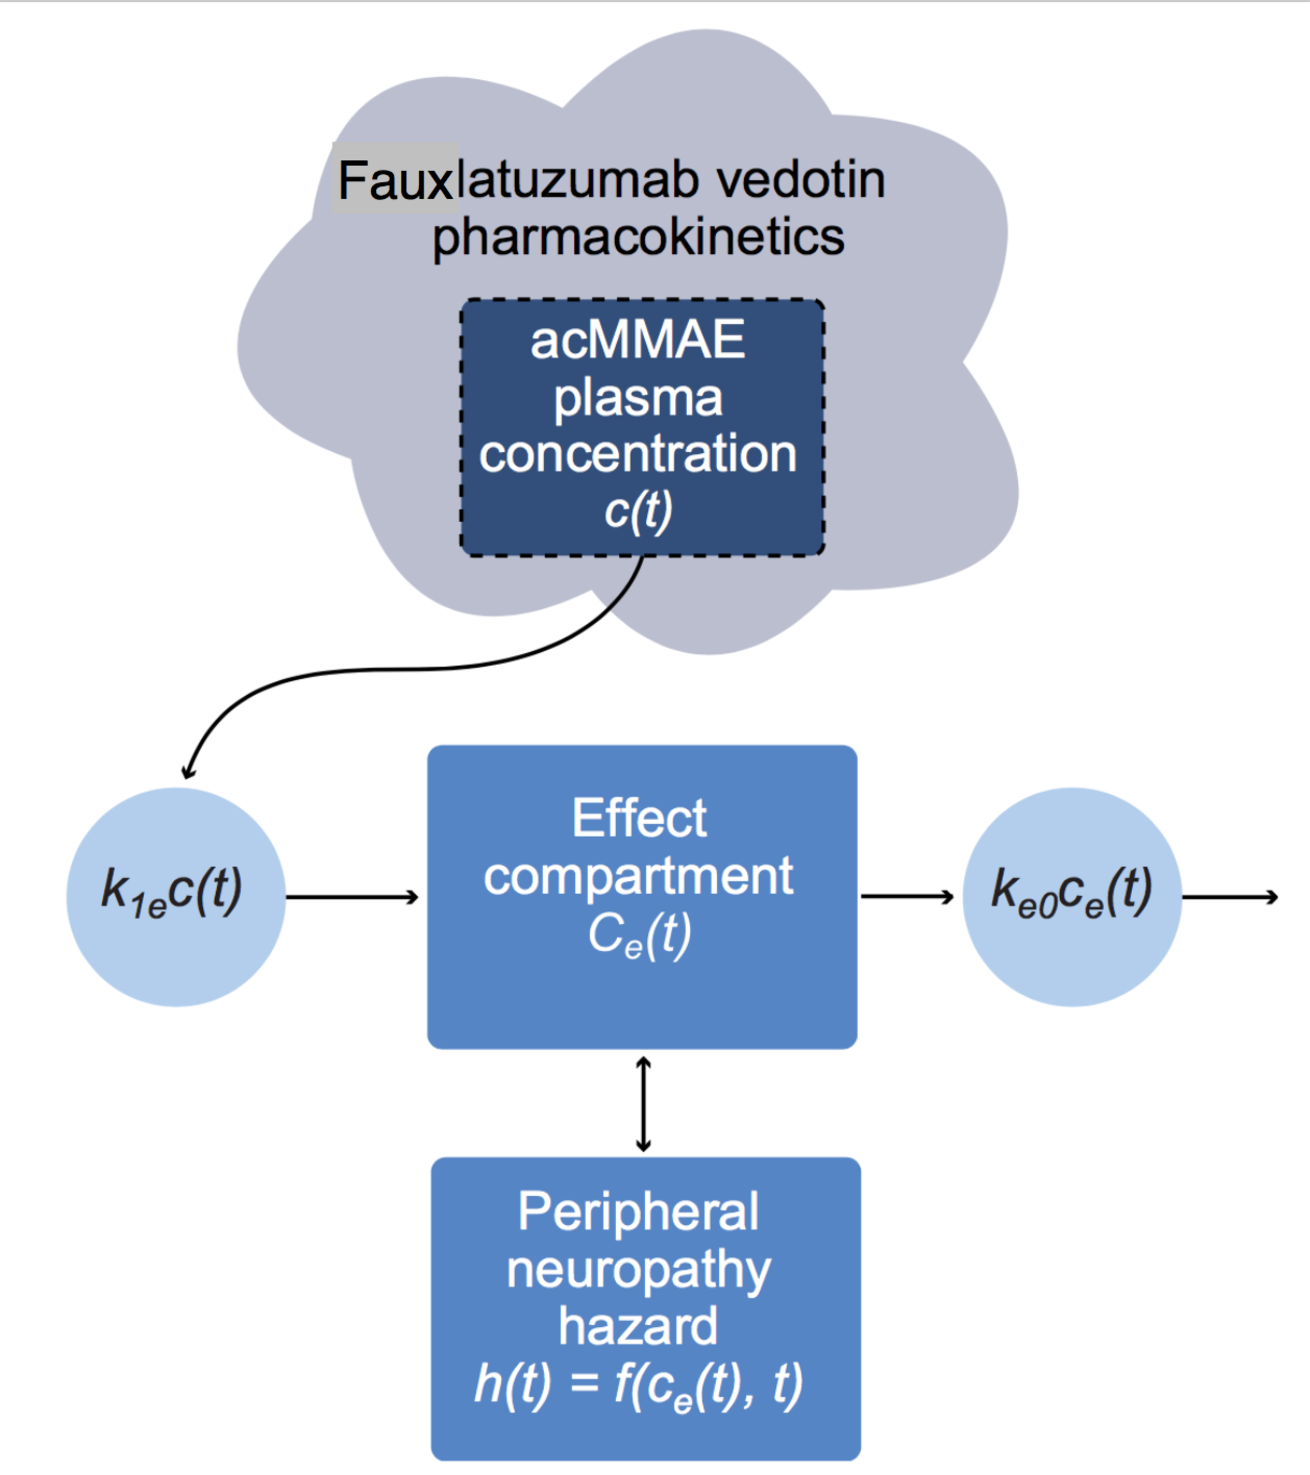
\includegraphics[width=0.9\columnwidth]{../../examples/ttpn2/lu2017Model.pdf}
\end{center}
\end{block}
\end{column}
\begin{column}{0.7\columnwidth}
\begin{block}{Note}
\begin{itemize}
\item To keep things simpler, we use the simulated individual CL and V values, and only model PD part of the problem.
\item PN hazard is substantially delayed relative to PK exposure.
\item Hazard increases over time to an extent not completely described by PK.
\end{itemize}
\end{block}
\end{column}
\end{columns}
\end{frame}

\begin{frame}[label={sec:orgd235adc}]{Exercise}
Likelihood for time to first PN \(\ge\) 2 event in the \(i^{th}\) patient:
\begin{align*}
\lefteqn{L\left(\theta | t_{\text{PN},i}, \text{censor}_i, X_i\right)} \\
  &= \left\{ \begin{array}{ll}
     h_i\left(t_{\text{PN},i} | \theta, X_i\right) e^{-\int_0^{t_{\text{PN},i}} h_i\left(u | \theta, X_i\right) du}, &
    \text{censor}_i = 0 \\
     e^{-\int_0^{t_{\text{PN},i}} h_i\left(u | \theta, X_i\right) du}, &
     \text{censor}_i = 1
\end{array} \right.
\end{align*}
where
 \begin{align*}
   t_{\text{PN}} &\equiv \text{time to first PN $\ge$ 2 or right
     censoring event} \\
 \theta &\equiv \text{model parameters} \\
 X &\equiv \text{independent variables / covariates} \\
 \text{censor} &\equiv \left\{ \begin{array}{ll}
     1, & \text{PN $\ge$ 2 event is right censored} \\
     0, & \text{PN $\ge$ 2 event is observed} 
 \end{array} \right.
\end{align*}
One can see the expression
\begin{equation*}
  e^{-\int_0^{t_{\text{PN},i}} h_i\left(u | \theta, X_i\right) du}
\end{equation*}
as the survival function at time \(t\).
\end{frame}

\begin{frame}[label={sec:orgd4a629d}]{Exercise}
Hazard of PN grade 2+ based on the Weibull distribution,
with drug effect proportional to effect site concentration of MMAE:
\begin{align*}
  h_j(t) &= \beta E_{\text{drug}j}(t)^\beta t^{(\beta - 1)} \\
  E_{\text{drug}j}(t) &= \alpha c_{ej}(t) \\
  c^\prime_{ej}(t) &= k_{e0} \left(c_j(t) - c_{ej}(t)\right).
\end{align*}

Overall ODE system including integration of the hazard function:
\begin{align}
  x_1^\prime &= -\frac{CL}{V} x_1 \\
  x_2^\prime &= k_{e0} \left(\frac{x_1}{V} - x_2\right) \\
  x_3^\prime &= h(t)
  \end{align}
where \(x_2(t) = c_e(t)\) and \(x_3(t) = \int_0^t h(u) du\) aka cumulative hazard.
\end{frame}

\begin{frame}[fragile,label={sec:orgc697d7a}]{Exercise}
 \begin{block}{"just walk in a minute ago, literally" mode}
\begin{itemize}
\item Apply \texttt{pmx\_solve\_group\_rk45} function.
\end{itemize}
\end{block}
\begin{block}{Intermediate mode}
\begin{itemize}
\item Code args for \texttt{pmx\_solve\_group\_rk45} function and
apply it. Use input data file \texttt{ttp2n.data2.R} as hint.
\end{itemize}
\end{block}
\begin{block}{hard mode}
\begin{itemize}
\item Code ODE
\item Code args for \texttt{pmx\_solve\_group\_rk45} function and
apply it. Use input data file \texttt{ttp2n.data2.R} as hint.
\item Code likelihood for harzard and censor event. Use
\texttt{model} block as hint.
\end{itemize}
\end{block}
\begin{block}{"why bother" mode}
\begin{itemize}
\item Code the model, use input data file \texttt{ttp2n.data2.R} 
and initial file \texttt{ttpn2.init.R} as hint.
\end{itemize}
\end{block}
\end{frame}
\begin{frame}[fragile,label={sec:org2aab45a}]{Exercise}
 \begin{block}{Edit/Add \texttt{cmdstan/make/local}}
\begin{minted}[breaklines=true,fontsize=\footnotesize,breakanywhere=true]{sh}
TORSTEN_MPI = 1         # flag on torsten's MPI solvers
CXXFLAGS += -isystem /usr/local/include # path to MPI library's headers
\end{minted}
\end{block}
\begin{block}{Build in \texttt{cmdstan}}
\begin{minted}[breaklines=true,fontsize=\footnotesize,breakanywhere=true]{sh}
make ../example-models/ttpn2/ttpn2_group
\end{minted}
\end{block}
\begin{block}{Run}
\begin{minted}[breaklines=true,fontsize=\footnotesize,breakanywhere=true]{sh}
mpiexec -n 4 -l ttpn2_group sample num_warmup=500 num_samples=500 data file=ttpn2.data2.R init=ttpn2.init.R
\end{minted}
\end{block}
\end{frame}

\begin{frame}[fragile,label={sec:orgb3a97a8}]{Exercise}
 \begin{itemize}
\item The parallel performance is not optimal, why?
\item Can you do it using Stan's \texttt{map\_rect}?
\end{itemize}
\end{frame}

\begin{frame}[label={sec:org0cf9e2e}]{Reference}
\bibliography{ttpn2}
\bibliographystyle{plain}
\end{frame}
\end{document}
